\documentclass[8pt,twocolumn,a4paper]{article}
\usepackage{ucs} 
\usepackage[left=2.5cm, right=2.5cm, top=2.0cm, bottom=2.5cm]{geometry}
\usepackage{amsmath,amssymb,amsfonts,amsthm}
\usepackage[utf8x]{inputenc} 
\usepackage[russian]{babel}
\usepackage{multicol}
\usepackage{fancyhdr}
\usepackage{indentfirst}
\usepackage[argument]{graphicx}
\usepackage[dvipsnames]{xcolor}
\graphicspath{}

\linespread{1.1}
\setlength\parindent{0ex}
\pagestyle{fancy}
\fancyhf{}
\rfoot{\huge\bfseries\page{79}}
\renewcommand{\headrulewidth}{0pt}

\begin{document}
\\\small
$OO_{1}^2=OD^2+O_{1}^2- 2 \cdot OD \cdot O_{1}D\cdot \cos{\angle ODO_{1}}$, где
$\angle ODO_{1} = \cfrac{2\pi}{3}$, дает уравнение для {\it r}, при решении которого надо учесть, что {\it r}$\geq0$. \newline
5.$-\cfrac{17}{48}.$   Р е ш е н и е. Из второго равенства получаем
\begin{center}
  $z=\cfrac{a}{3} - \cfrac{x}{3} - \cfrac{2y}{3}$  
\end{center}

 с учетом этого из первого получаем уравнение
\begin{center}
    \large$(x-\frac{1}{3})^2+(2y-\frac{1}{12})^2 = \frac{a}{3} + \frac{17}{144}.$
\end{center}
правая часть которого должна быть равна нулю.

\newline
\textbf{Физика} \newline \newline
\textbf{1.} \large$h= \frac{g\tau^2}{2}(\sqrt{(\frac{F}{mg})^2-\cos^2{a}}-\sin{a})\sin{a}.$ \newline
\textbf{2.} $\Delta h= m/(2\varrho S).$ \newline
\textbf{3.} $\mu=\cfrac{\cos{\varphi_{1}}-\cos{\varphi_{0}}} {\sin{\varphi_{1}}+ \sin{\varphi_{0}}}tg{\alpha} \approx \cfrac{\varphi_{0}-\varphi_{1}}{2}tg{\alpha}.$ \newline
\textbf{4.} $A= RT/4.      $ \newline
\textbf{5.} \large $r_{2} = \cfrac{\rho_{H1}T_{2}}{\rho_{H1}T_{1}}r_{1}$ + $\cfrac{mRT_{2}}{\mu V \rho_{H2}} \approx 58\%$ \newline \text{(здесь} $\rho_{H2} \approx 10^5$ \text{Па, } $\mu = 18 \cdot 10^{-3}$ \text{кг/моль).} \newline
\textbf{6.} $\varphi_{0} = (C_{1}\varphi_{1}+C_{2}\varphi_{2}+C_{3}\varphi_{3}+)/(C_{1}+C_{2}+C_{3}). $
\newline\textbf{7.} $ Q=C\Im^{2} / 12. $ \newline
\textbf{8.} $ \Im = \cfrac{R_{2}-R_{1}}{    \sqrt{R_{2}/P_{2}} - \sqrt{R_{1}/P_{1}}             } .  $ \newline
\textbf{9.} $ \delta = \varphi - \pi / 2 + \arcsin{ \sqrt{\pi^2-\sin^2{\varphi}}    } . $ \newline
\textbf{10.} $F=-ld_{1}/d_{2}= -20 $ \text{см.} \newline


\textbf{\small«Квант» для младших школьников} \newline
\chapter{\small(см. «Квант» №1)} \newline
%\text{(см. «Квант» №1)}
\newline
\textbf{\small1.}  \text{\smallДа, был.}                      \newline
\textbf{\small2.}                \text{\smallПервую и третью девочку}        \newline
\textbf{\small3.} \smallПусть $\alpha$ и $b$ - искомые числа. Тогда  $\alpha-b=n$ и $\alpha=nb.$ Отсюда $b(n-1)=n$ или $$ b=\frac{n}{n-1}=1+\frac{1}{n-1} .$$           
Так как b - натуральное, то n=2, b=2 и $\alpha=4$. \newline
\textbf{\small4.}           \text{\smallСм. рис. 13.}             \newline
\textbf{\small5.}             \text{\small11 оборотов}           

\newline

\begin{center}

\begin{tabular}{ | l | l | l | l | l |}
\hline
К & О & Р & А & Н \\ \hline
Н & Р & А & К & О \\ \hline
А & К & О & Н & Р \\ \hline
О & А & Н & Р & К \\ \hline
Р & Н & К & О & А \\
\hline
\end{tabular}

\end{center}
\newline \newline \newline

\text{\smallРис.13.} \newline
\newline

\textbf{\small Избранные задачи Ленинградской городской математичской олимпиады 1989 года} \newline
\chapter{\small(см. «Квант» №1)}
\\ \small
1. Решение единственно - это числа 166667 и 33334. \newline 2. Выигрывает второй игрок. Его стратегия такова: отвечать на симметричное относительно центра доски поле другим знаком, за исключением тех случаев, когда еть прямо выигрывающий ход.\newline 3. После вычитания второго уравнения из первого получаем $(A-B)^2+(B-C)^2=0 $, откуда вытекает, что есть два решения $A=B=C= \pm 10$. \newline 4.Если у нашего числа есть простые делители, большие 3, то оно не меньше 3000. Но уже число $2^{11}=2048$, очевидно, удовлетворяет требованиям задачи. Значит, искомое число не больше 2048 и не может иметь делителей, больших 3. Поэтому его надо искать среди чисел вида $2^k\cdot3^t$. \newline 5. Количество физиков за столом равно количеству лжецов, а оно четно. \newline 6. Второй ставит фишку в симметричное относительно центра доски поле. Докажите (это чисто геометрический факт), что его ход всегда длиннее предыдущего хода первого игрока.\newline 7. Рассмотри любой набор из различных натуральных чисел, например 1,2, ...,100. Умножим все числа на одно и то же число А, делящееся на все возможные суммы пятерок, набор $500!, 2\cdot500!, 3\cdot500!, ..., 100\cdot500!$ - проверьте, что это и есть требуемый набор. \newline 8. Пусть $B-K=k$,Тогда $A^{2}+1=(A+k)\times(A-k)+k^2+1 $, и значит, $k^2+1$ делится на B, т.е. $ k^2+1\geq B$, или $k^2\geq B-1 >A$(случай $B=A+1$ по условию не возможен). \newline 9. Так как $x+y+z=0$ и $xy+xz+yz=0 $, то $(x+y+z)^2 - 2(xy+xz+yz)=x^2+y^2+z^2=0$, т.е. $x=y=z=0$, что невозможно. \newline 10. а) 2; б) 2 или 3. Очевидно, что 2 участника могли провести подобный турнир. Рассмотрим темерь победителя турнира- он насбрал не более $k(n-1)$ очков (если всего n участников). Все остальные набрали не менее $k(n-1)(n-2)/2$ очков. С другой стороны, если знаминатель прогресии равен q, то победитель должен набрать более чем в $q-1$ раз больше очков, чем все остальные участники. Отсюда следует общий результат: если $k$ не делится на 7, то $n=2$; если $k$ делится на 7, то $n=2$ или 3. \newline 11. Обратите внимание на то, что все пять треугольников, расположенных в вершинах звезды,- это подобные равнобедренные треугольники. \newline 12. Ответ положительный. Доказательство легко проводится индукцией для всех таблиц вида $2n\times2n$. \newline 13. Рассмотрите грани, примыкающие к самому короткому боковому ребру. \newline 14. Используя свойства операции $\ast$, получаем $ (c\ast\alpha)\ast b = -b\ast(c\ast\alpha)= -(b\ast c)\ast\alpha=\alpha\ast(b\ast c)= (\alpha\ast b)\ast c= -c\ast(\alpha\ast b)= -(c\ast\alpha)\ast b$. Отсюда следует, что    $x\ast y $ всегда равно 0. \newline Обозначим центр описанной около BMC окружности через O. Докажите, что ABOC- вприсанный четырехугольник.Отсюда нетрудно вывести, что AM-

\newpage



\linespread{1.1}
\setlength\parindent{0ex}
\pagestyle{fancy}
\fancyhf{}
\rfoot{\huge\bfseries\page{80}}
\renewcommand{\headrulewidth}{0pt}
\DeclareGraphicsExtensions{.pdf,.png,.jpg}

\hfil
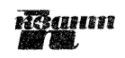
\includegraphics[width=40mm]{kvok.jpg} \newline

\textbf{\largeГлавный редактор -} \newline  \text{\largeакадемик Ю.Осипьян } \newline \newline

%\itshape\\[80pt]
%\raisebox{\textup{\texttt{\huge "КЛЮЧ$"$   К РЕШЕНИЮ - ПОДОБНЫЕ ТРЕУГОЛЬНИКИ}}}
\begin{minipage}{0.08\textwidth}

\fbox { \parbox[t][25]{110mm}{ \itshape\\ [120pt]\raisebox{\textup{}{\textit{\color{Black}\bfseries\Huge Ш\color{Goldenrod}а\color{Black}х\color{Goldenrod}м\color{Black}а\color{Goldenrod}т\color{Black}н\color{Goldenrod}а\color{Black}я \color{Goldenrod}с\color{Black}т\color{Goldenrod}р\color{Black}а\color{Goldenrod}н\color{Black}и\color{Goldenrod}ч\color{Black}к\color{Goldenrod}а }}}}}
\end{minipage}


\end{document}